
\documentclass[preprint,12pt]{elsarticle}

\usepackage[spanish]{babel}
\usepackage{amssymb}
\usepackage{graphicx}
\usepackage{lineno}
\usepackage[utf8]{inputenc}
\usepackage{url}



\begin{document}
	
	\begin{frontmatter}
		
		
		\title{\huge Balanced ScoreCard y Business Model Canvas}
		
		\author{Mamani Ayala, Brandon        (2015052715)}
		\author{Quispe Mamani, Angelo	      (2015052826)}
		\author{Vizcarra Llanque, Jhordy	      (2015052719)}
		\author{Ordoñez Quilli, Ronald          (2015052821)}
		\author{Rodriguez Mamani, Juan      (2017057862)}
		
		\address{Tacna, Perú}
		
		\begin{abstract}
			%% Text of abstract
			Performance Management bevat activiteiten die ervoor kunnen zorgen dat doelen consistent worden behaald op een effectieve en efficiënte wijze. Middels het Business Model Canvas wordt u een concept aangeboden, waarmee u het business model van uw organisatie kunt beschrijven, overdenken en onderzoeken. Een business model kan het beste worden beschreven aan de hand van negen basisbouwstenen, die de logica laten zien van hoe een bedrijf geld wil gaan verdienen.
Na een strategische heroriëntatie in een snel veranderende omgeving, gaan wij verder in op de best practice in performance management, de Business Balanced Scorecard (‘BSC’). De nadruk ligt op de praktische implementatie van de BSC en het bouwen van een gebalanceerde dashboard, waarbij niet alleen rekening wordt gehouden met een financial dashboard, maar ook met het klantperspectief, intern en innovatief perspectief.
	
		\end{abstract}
\end{frontmatter}
%%

	
	%%
	%\linenumbers
	
	%% main text
	
	%%
	%\linenumbers
	
	%% main text



\section{Balanced ScoreCard }

\title{Balanced Scorecard}
El Balanced Scorecard (BSC / Cuadro de Mando Integral) es una herramienta que permite enlazar estrategias y objetivos clave con desempeño y resultados a través de cuatro áreas críticas en cualquier empresa: desempeño financiero, conocimiento del cliente, procesos internos de negocio y aprendizaje y crecimiento. \\
Sin embargo, es algo más que un nuevo sistema de medición. Las empresas innovadoras utilizan el Cuadro de Mando integral como el marco y estructura central y organizativa para sus procesos. Las empresas pueden desarrollar un Cuadro de mando Integral, con unos objetivos bastante limitados: conseguir clarificar, obtener el consenso y centrarse en su estrategia, y luego comunicar esa estrategia a toda la organización. Sin embargo, el verdadero poder del Cuadro de mando Integral aparece cuando se transforma de un sistema de indicadores en un sistema de gestión. A medida que más y más empresas trabajan con el 
Cuadro de Mando Integral, se dan cuenta de que puede utilizarse para:
		\begin{itemize}
		\item Clarificar la estrategia y conseguir el consenso sobre ella.
		\item Comunicar la estrategia a toda la organización.
		\item Alinear los objetivos personales y departamentales con la estrategia.
		\item Vincular los objetivos estratégicos con los objetivos a largo plazo y los presupuestos anuales.
		\item Identificar y alinear las iniciativas estratégicas.
		\item Realizar revisiones estratégicas periódicas y sistemáticas
		\item Obtener feedback para aprender sobre la estrategia y mejorarla.
		\end{itemize}

\begin{center}
	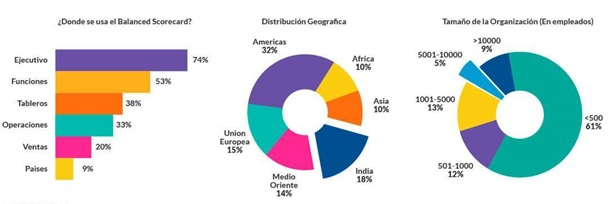
\includegraphics[width=12cm]{./Imagenes/img1} 
\end{center}

El cuadro de mando integral llena el vacío que existe en la mayoría de sistemas de gestión: la falta de un proceso sistemático para poner en práctica la estrategia y obtener feedback sobre ella. Los procesos de gestión alrededor del Cuadro de Mando permiten que la organización se equipare y se centre en la puesta en práctica de la estrategia a largo plazo. Utilizado de este modo, el Cuadro de Mando Integeral se convierte en los cimientos para gestionar las organizaciones de la era de la información.\\
\\
En la siguiente figura se presentan las cuatro perspectivas del Cuadro de Mando Integral, se puede apreciar que es un sistema que considera todos los procesos estratégicos de la organización:

\begin{center}
	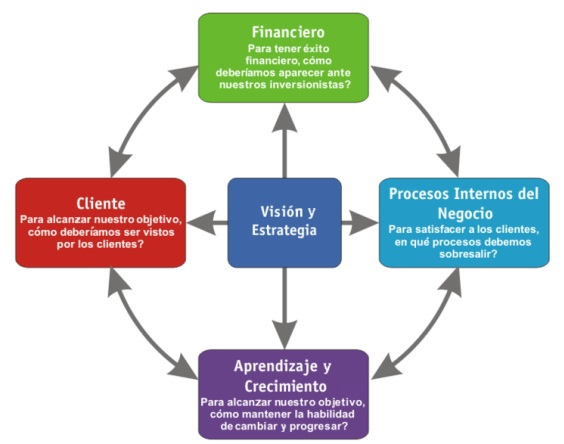
\includegraphics[width=10cm]{./Imagenes/img2} 
\end{center}

Balanced Scorecard, ejemplo de mapa estratégico de una joyería

\begin{center}
	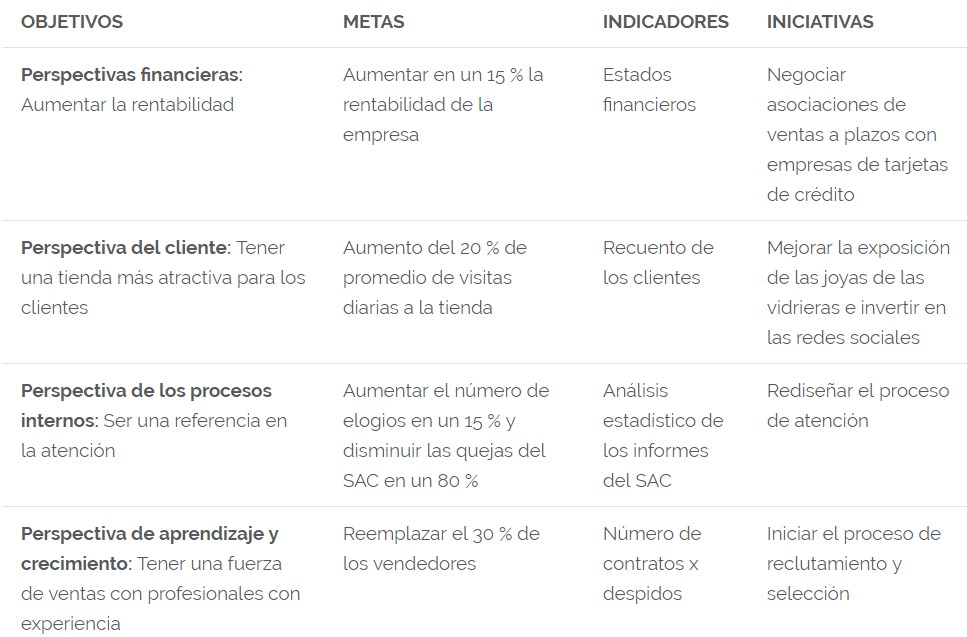
\includegraphics[width=13cm]{./Imagenes/img3} 
\end{center}

Areas críticas de Balanced Scorecard:
		\begin{itemize}
		\item Indicadores desde la perspectiva de los procesos internos: Desde esta perspectiva son analizados aquellos procesos de la empresa que están dirigidos a obtener el rendimiento esperado en los tiempos programados. Así, este grupo de indicadores incluye aquellos que están relacionados con la calidad del proceso, como son los indicadores de productividad, de calidad del producto, de costos del producto, de eficiencia del proceso de fabricación.

Igualmente, serán considerados en este grupo los indicadores de tiempos de entrega, de calidad de materias primas, de mantenimiento de productos, así como los indicadores medioambientales.
		\item Indicadores desde la perspectiva del cliente: En este grupo se encuentran los indicadores relacionados con las soluciones destinadas a satisfacer las necesidades de los clientes. También se consideran aquellos vinculados a mejorar la cuota de mercado de la empresa.

Entre dichos indicadores se encuentran la fidelidad del cliente, la satisfacción del cliente, la calidad  que se percibe de nuestro producto o servicio, la imagen que los clientes tienen de la empresa, la calidad del servicio postventa y del servicio de atención al cliente.

		\item Indicadores desde la perspectiva financiera: Aquí se consideran los indicadores analizados desde la contabilidad y las finanzas, especialmente aquellos que dan cuenta de la situación económica de la empresa. Entre dichos indicadores podemos considerar las ampliaciones de capital, las fusiones o absorciones, la emisión de acciones, bonos u otros instrumentos financieros y la creación de filiales.

También integran este grupo de indicadores la gestión del riesgo, la liquidez de la empresa, el endeudamiento, etc.

		\item Indicadores desde la perspectiva de la innovación y aprendizaje: En este cuarto grupo de indicadores se considera aquellos relacionados con la introducción de innovación en los diversos procesos de la organización, la capacitación de los trabajadores, ventas por lanzamiento de nuevos productos o servicios, ahorros de costos por innovación en procesos, ROI por la inversión en innovación, ratio de éxito de nuevos productos, incremento de capacidades en el personal, etc.

La implementación y análisis de estos indicadores en la forma de cuadro de mando integral permitirá realizar el control de diversos aspectos estratégicos de la organización, lo cual llevará a tomar decisiones relacionadas con acciones preventivas y correctivas, así como de mejoramiento del rendimiento mediante la implementación de las cuatro perspectivas señaladas.
	\end{itemize}


Ventajas de Balanced Scorecard:
\begin{itemize}
		\item Permite tener una visión y control de cómo el funcionamiento de cada área y miembro de la empresa influye en el resto de la organización.
		\item Establecer una vinculación entre los objetivos de la empresa y las acciones necesarias para lograrlos.
		\item Una vez ejecutadas las acciones de mejora, detectar cómo influyen en otras áreas de la empresa, lo que permitirá ejecutar correcciones adicionales si es necesario.
		\item Implantar un modelo de gestión flexible e interactivo, acorde a los actuales requerimientos y exigencias del mercado.
		\item Incorporación de perspectivas distintas a las financieras, como la perspectiva del cliente o la interna o de procesos de negocio.
		\item Disponer de una una imagen muy clara y gráfica del status de la organización en cada momento en cuanto a metas, resultados y acciones en desarrollo o ya implantadas.
		\item Ayuda a tomar las decisiones más acertadas en el momento oportuno para maximizar la rentabilidad y productividad de la empresa.
		\item Facilita la comunicación entre dirección, mandos intermedios y empleados para que todos tenga una idea muy clara de los objetivos, específicos y generales, de la empresa y de las acciones necesarias para lograrlos.
	\end{itemize}


	%%
	
	%%
	%\linenumbers
	
	%% main text

\section{Marco Teorico}
	
\subsection{subtitulo}	

	aqui el marco teorico 
		
\subsection{subtitulo2}
		
	

	%%
	%\linenumbers
	
	%% main text


%%
	
	%%
	%\linenumbers
	
	%% main text
\section{Conclusion}
aqui la conclusion

%%
	
	%%
	%\linenumbers
	
	%% main text

	
	
	\newpage
	
	\bibliographystyle{apalike} 	%ESTILO
	\bibliography{BIBLIOGRAFIA}		%ARCHIVO .bib
	
	%% The Appendices part is started with the command \appendix;
	%% appendix sections are then done as normal sections
	%% \appendix
	
	%% \section{}
	%% \label{}
	
	%% References
	%%
	%% Following citation commands can be used in the body text:
	%% Usage of \cite is as follows:
	%%   \cite{key}          ==>>  [#]
	%%   \cite[chap. 2]{key} ==>>  [#, chap. 2]
	%%   \citet{key}         ==>>  Author [#]
	
	%% References with bibTeX database:
	
	
	%% Authors are advised to submit their bibtex database files. They are
	%% requested to list a bibtex style file in the manuscript if they do
	%% not want to use model1-num-names.bst.
	
	%% References without bibTeX database:
	
	% \begin{thebibliography}{00}
	
	%% \bibitem must have the following form:
	%%   \bibitem{key}...
	%%
	
	% \bibitem{}
	
	% \end{thebibliography}
	
	
\end{document}

%%
%% End of file `elsarticle-template-1-num.tex'.
